%%
%% (
%%  )\ )                             (
%%  (()/(   (            (             )\  )   (
%%   /(_))  ))\   (       ))\  (   (   (()/(   ))\
%%   (_))  /((_)  )\  )  /((_) )\  )\   ((_))/((_)
%%   | _ \(_))(  _(_/( (_) )  ((_)((_)  _| |(_))
%%   |   /| || || ' \))/ -_)/ _|/ _ \/ _` |/ -_)
%%   |_|_\ \_,_||_||_| \___|\__|\___/\__,_|\___|
%%

\documentclass{article}
\usepackage{fontspec}
\usepackage[utf8]{inputenc}
\usepackage{amsmath}
%\usepackage{slashbox}
\usepackage{amsfonts}
\usepackage{amssymb}
\usepackage{graphicx} % Paquete para incluir imágenes en el documento LaTeX
\usepackage{hyperref}
\hypersetup{
  colorlinks=true,
  linkcolor=blue,
  filecolor=magenta,
  urlcolor=cyan,
}
\urlstyle{same}
\usepackage{varwidth}

\newcommand\tab[1][1cm]{\hspace*{#1}}

\usepackage{multirow}

\usepackage[a4paper,rmargin=1.5cm,lmargin=1.5cm,top=1.5cm,bottom=1.5cm]{geometry}

\usepackage{pdfpages}

\usepackage{xcolor}
\usepackage{minted}
\setminted[css]{frame=lines, framesep=2mm, baselinestretch=1.2, rulecolor=\color{black!80},
                bgcolor=DarkGray,fontsize=\normalsize}
\usemintedstyle[css]{monokai}
\setminted[python]{frame=lines, framesep=2mm, baselinestretch=1.2, rulecolor=\color{black!80}, bgcolor=DarkGray}
\usemintedstyle[python]{monokai}
\setminted[java]{frame=lines, framesep=2mm, baselinestretch=1.2, rulecolor=\color{black!80}, bgcolor=DarkGray}
\usemintedstyle[java]{monokai}
\setminted[javascript]{frame=lines, framesep=2mm, baselinestretch=1.2, rulecolor=\color{black!80}, bgcolor=DarkGray}
\usemintedstyle[javascript]{monokai}
\setminted[php]{frame=lines, framesep=2mm, baselinestretch=1.2, rulecolor=\color{black!30}, bgcolor=LightGray}
\setminted[html]{frame=lines, framesep=2mm, baselinestretch=1.2, rulecolor=\color{black!30}, bgcolor=LightGray}
\setminted[bash]{baselinestretch=1.2,rulecolor=\color{black!30},bgcolor=LightGray}
\definecolor{LightGray}{gray}{0.98}
\definecolor{DarkGray}{gray}{0.1}
\definecolor{MidGray}{gray}{0.8}
\definecolor{codegreen}{rgb}{0,0.6,0}
\definecolor{codegray}{rgb}{0.5,0.5,0.5}
\definecolor{codepurple}{rgb}{0.58,0,0.82}
\definecolor{backcolour}{rgb}{0.95,0.95,0.92}
\setminted[json]{frame=lines, framesep=2mm, baselinestretch=1.2, rulecolor=\color{black!80}, bgcolor=DarkGray}
\usemintedstyle[json]{monokai}
\setminted[apacheconf]{frame=lines, framesep=2mm, baselinestretch=1.2, rulecolor=\color{black!30}, bgcolor=LightGray}
\setminted[html+twig]{frame=lines, framesep=2mm, baselinestretch=1.2, rulecolor=\color{black!30}, bgcolor=LightGray}
\setminted[html+php]{frame=lines, framesep=2mm, baselinestretch=1.2, rulecolor=\color{black!30}, bgcolor=LightGray}

%\setlength{\parindent}{0px}  % Setea la indentacion de la primera linea de cada parrafo a cero pixeles.


\title{Programación en Laravel}
\author{@RuneCode}

\begin{document}

%% Clase 1
\section{Intro y características}%
Laravel es un framework completo que cuenta con muchos módulos que te ayudarán
para el desarrollo de tus aplicaciones. Existen otros frameworks de PHP como
Symfony o Zend, sin embargo Laravel es uno de los líderes en el mercado.\\

Laravel no solo es sencillo y tiene muchas herramientas de desarrollo, sino que
también cuenta con una amplia comunidad a su alrededor; esta comunidad ha
logrado que sea posible tener una excelente documentación que puede ser
encontrada en Laracast y se ha creado un gran ecosistema con foros y
comunidades.\\
También existen proyectos que se han desarrollado a partir de Laravel como
Lumen que es un micro-framework o Spark que te da un punto de inicio para
aplicaciones de cobros.\\

En este curso se trabajará pensando que ya tienes bases de PHP. Si no tienes
estas bases, puedes adquirirlas en el curso de Platzi de Introducción a PHP.\\
El proyecto del curso será crear un sistema para reporte de gastos.\\

%% Clase 2
\section{Instalación de Laravel}%
Composer es un manejador de dependencias para PHP, así que todas las
dependencias que necesitemos, incluído Laravel, serán instaladas por
Composer.
Para trabajar en Laravel necesitarás un servidor de PHP y una base de datos.\\
Laravel nos ofrece un instalador que podemos traer a través de Composer y
utilizaremos global en el comando para que la instalación se realice en toda la
máquina virtual o computador.
Podemos comprobar si Laravel quedó bien instalado usando el comando "laravel"
el cual nos dará la versión del instalador y los comandos disponibles.
El comando "new" nos ayuda a crear un nuevo proyecto de Laravel; al hacer esto
se crearán las carpetas y estructura del proyecto y el archivo composer con las
dependencias necesarias.
Para trabajar con Laravel es necesario tener la versión de PHP 7.1 o
superior.
El comando "artisan" nos da una serie de comandos de Laravel, son muchos y no
todos se utilizan pero es buena idea revisar la documentación y opciones
disponibles.
El comando "serve" levanta un servidor de PHP corriendo el proyecto actual, el
cual nos arroja una dirección IP la cual abriéndola nos muestra nuestro
proyecto.\\


\begin{figure}[h!]
  \centering
  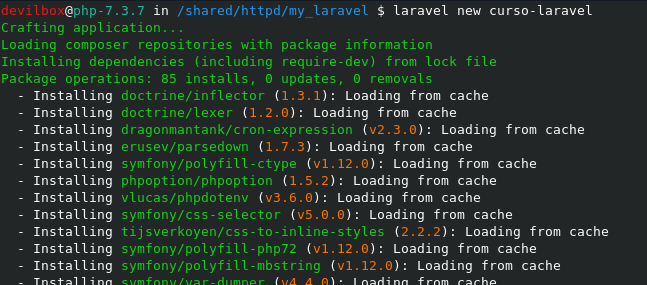
\includegraphics[scale=0.75]{./Pictures/001_Install_laravel.png}
\end{figure}

\begin{figure}[h!]
  \centering
  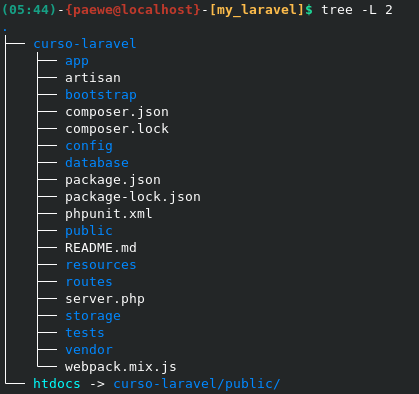
\includegraphics[scale=0.65]{./Pictures/002_estructura.png}
\end{figure}

\newpage

\begin{figure}[h!]
  \centering
  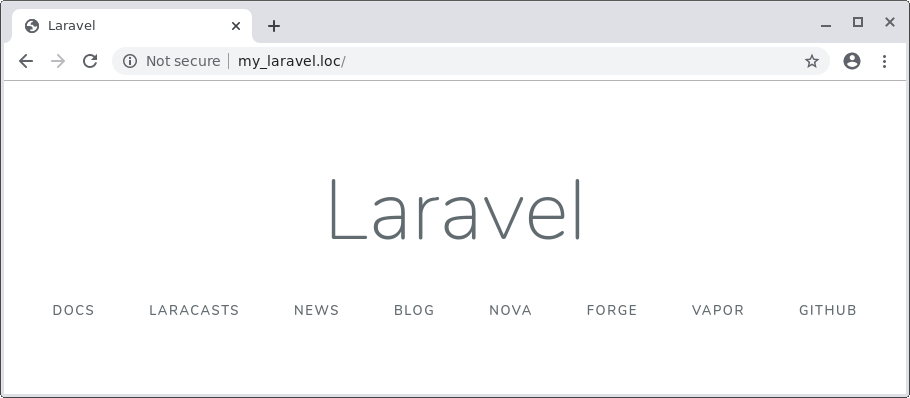
\includegraphics[scale=0.5]{./Pictures/003_laravel.png}
\end{figure}


%% Clase 3
\section{Primera ruta en Laravel}%
Laravel cuenta con un mecanismo para generar rutas y especificar el método que
queremos utilizar (get, post, put…) teniendo la posibilidad de incluso
mezclarlos.\\

\begin{itemize}
  \item En el archivo web.php encontramos todas las rutas que trabajaremos.
  \item Las vistas se encuentran dentro de resources/views.
  \item Las vistas básicas se realizan utilizando closures.
  \item Podemos regresar vistas, textos, arreglos asociativos, entre otros;
    devolviendo los arreglos en formato json lo cual es muy útil al momento de
    realizar pruebas.
  \item Es en web.php donde podemos definir el método que vamos a usar.
\end{itemize}


\textbf{routes/web.php}
\begin{minted}{php}
  <?php

  /*
  |--------------------------------------------------------------------------
  | Web Routes
  |--------------------------------------------------------------------------
  |
  | Here is where you can register web routes for your application. These
  | routes are loaded by the RouteServiceProvider within a group which
  | contains the "web" middleware group. Now create something great!
  |
  */

  Route::get('/', function () {
      return view('welcome');
  });

  Route::get('/test', function () {
    return "Hola Platzi";
  });
\end{minted}


\begin{figure}[h!]
  \centering
  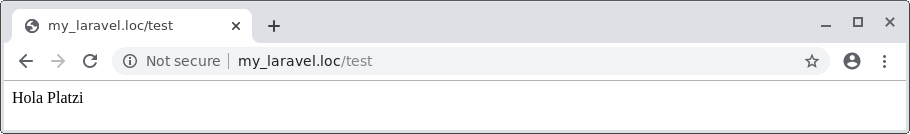
\includegraphics[scale=0.5]{./Pictures/004_test.png}
\end{figure}

\textbf{routes/web.php}
\begin{minted}{php}
  <?php

  /*
  |--------------------------------------------------------------------------
  | Web Routes
  |--------------------------------------------------------------------------
  |
  | Here is where you can register web routes for your application. These
  | routes are loaded by the RouteServiceProvider within a group which
  | contains the "web" middleware group. Now create something great!
  |
  */

  Route::get('/', function () {
      return view('welcome');
  });

  Route::get('/test', function () {
    return [
      'saludo' => 'Hola',
      'nombre' => 'Platzi'
    ];
  });
\end{minted}

\begin{figure}[h!]
  \centering
  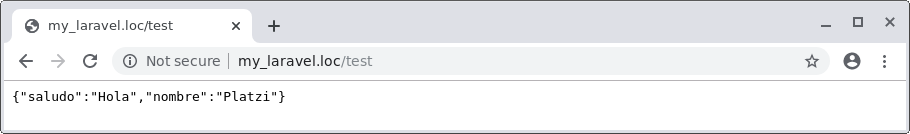
\includegraphics[scale=0.5]{./Pictures/005_laravel_json.png}
\end{figure}

\textbf{resources/views/welcome.blade.php}
\begin{minted}{html+php}
  <!DOCTYPE html>
  <html lang="{{ str_replace('_', '-', app()->getLocale()) }}">
      <head>
          <meta charset="utf-8">
          <meta name="viewport" content="width=device-width, initial-scale=1">

          <title>Laravel</title>

          <!-- Fonts -->
          <link href="https://fonts.googleapis.com/css?family=Nunito:200,600" rel="stylesheet">

          <!-- Styles -->
          <style>
              html, body {
                  background-color: #fff;
                  color: #636b6f;
                  font-family: 'Nunito', sans-serif;
                  font-weight: 200;
                  height: 100vh;
                  margin: 0;
              }

              .full-height {
                  height: 100vh;
              }

              .flex-center {
                  align-items: center;
                  display: flex;
                  justify-content: center;
              }

              .position-ref {
                  position: relative;
              }

              .top-right {
                  position: absolute;
                  right: 10px;
                  top: 18px;
              }

              .content {
                  text-align: center;
              }

              .title {
                  font-size: 84px;
              }

              .links > a {
                  color: #636b6f;
                  padding: 0 25px;
                  font-size: 13px;
                  font-weight: 600;
                  letter-spacing: .1rem;
                  text-decoration: none;
                  text-transform: uppercase;
              }

              .m-b-md {
                  margin-bottom: 30px;
              }
          </style>
      </head>
      <body>
          <div class="flex-center position-ref full-height">
              @if (Route::has('login'))
                  <div class="top-right links">
                      @auth
                          <a href="{{ url('/home') }}">Home</a>
                      @else
                          <a href="{{ route('login') }}">Login</a>

                          @if (Route::has('register'))
                              <a href="{{ route('register') }}">Register</a>
                          @endif
                      @endauth
                  </div>
              @endif

              <div class="content">
                  <div class="title m-b-md">
                      Curso Laravel
                  </div>

                  <div class="links">
                      <a href="https://laravel.com/docs">Docs</a>
                      <a href="https://laracasts.com">Laracasts</a>
                      <a href="https://laravel-news.com">News</a>
                      <a href="https://blog.laravel.com">Blog</a>
                      <a href="https://nova.laravel.com">Nova</a>
                      <a href="https://forge.laravel.com">Forge</a>
                      <a href="https://vapor.laravel.com">Vapor</a>
                      <a href="https://github.com/laravel/laravel">GitHub</a>
                  </div>
              </div>
          </div>
      </body>
  </html>
\end{minted}

\begin{figure}[h!]
  \centering
  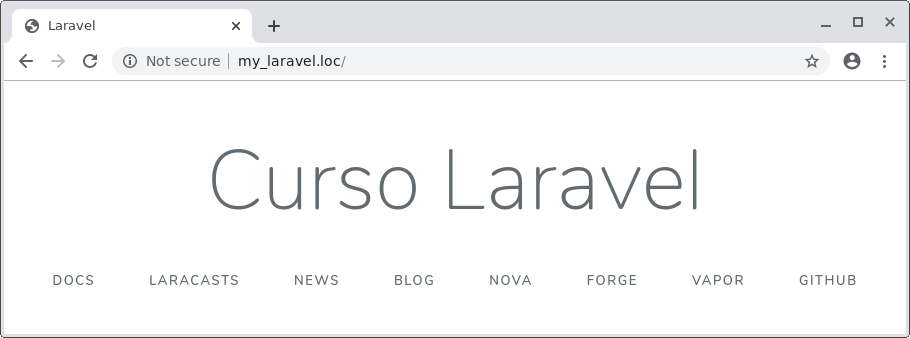
\includegraphics[scale=0.5]{./Pictures/006_vistas.png}
\end{figure}

\textbf{routes/web.php}
\begin{minted}{php}
  <?php

  /*
  |--------------------------------------------------------------------------
  | Web Routes
  |--------------------------------------------------------------------------
  |
  | Here is where you can register web routes for your application. These
  | routes are loaded by the RouteServiceProvider within a group which
  | contains the "web" middleware group. Now create something great!
  |
  */

  Route::get('/', function () {
      return view('welcome');
  });

  Route::get('/test', function () {
    return view('test');
  });
\end{minted}

\textbf{resources/views/test.blade.php}
\begin{minted}{php}
  <!DOCTYPE html>
  <html lang="{{ str_replace('_', '-', app()->getLocale()) }}">
      <head>
          <meta charset="utf-8">
          <meta name="viewport" content="width=device-width, initial-scale=1">

          <title>Laravel</title>

          <!-- Fonts -->
          <link href="https://fonts.googleapis.com/css?family=Nunito:200,600" rel="stylesheet">

          <!-- Styles -->
          <style>
              html, body {
                  background-color: #fff;
                  color: #636b6f;
                  font-family: 'Nunito', sans-serif;
                  font-weight: 200;
                  height: 100vh;
                  margin: 0;
              }

              .full-height {
                  height: 100vh;
              }

              .flex-center {
                  align-items: center;
                  display: flex;
                  justify-content: center;
              }

              .position-ref {
                  position: relative;
              }

              .top-right {
                  position: absolute;
                  right: 10px;
                  top: 18px;
              }

              .content {
                  text-align: center;
              }

              .title {
                  font-size: 84px;
              }

              .links > a {
                  color: #636b6f;
                  padding: 0 25px;
                  font-size: 13px;
                  font-weight: 600;
                  letter-spacing: .1rem;
                  text-decoration: none;
                  text-transform: uppercase;
              }

              .m-b-md {
                  margin-bottom: 30px;
              }
          </style>
      </head>
      <body>
          <div class="flex-center position-ref full-height">
              @if (Route::has('login'))
                  <div class="top-right links">
                      @auth
                          <a href="{{ url('/home') }}">Home</a>
                      @else
                          <a href="{{ route('login') }}">Login</a>

                          @if (Route::has('register'))
                              <a href="{{ route('register') }}">Register</a>
                          @endif
                      @endauth
                  </div>
              @endif

              <div class="content">
                  <div class="title m-b-md">
                      Curso Laravel en Platzi
                  </div>

                  <div class="links">
                      <a href="https://laravel.com/docs">Docs</a>
                      <a href="https://laracasts.com">Laracasts</a>
                      <a href="https://laravel-news.com">News</a>
                      <a href="https://blog.laravel.com">Blog</a>
                      <a href="https://nova.laravel.com">Nova</a>
                      <a href="https://forge.laravel.com">Forge</a>
                      <a href="https://vapor.laravel.com">Vapor</a>
                      <a href="https://github.com/laravel/laravel">GitHub</a>
                  </div>
              </div>
          </div>
      </body>
  </html>
\end{minted}

\begin{figure}[h!]
  \centering
  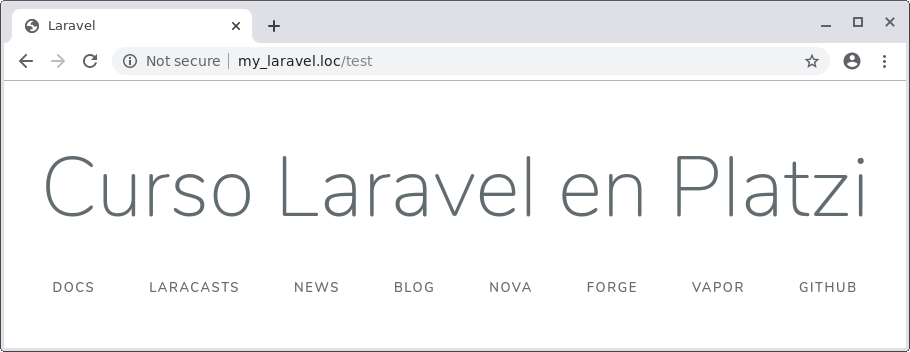
\includegraphics[scale=0.5]{./Pictures/007_test_vistas.png}
\end{figure}


%% Clase 4
\section{Cómo funciona Blade}%
Internamente Laravel utiliza un motor de render llamado Blade y utilizamos este
tipo motores porque PHP ha ido evolucionando más su parte de programación pero
no tanto su parte de motores de templates. Algunas librerías han sido creadas
para solventar esa falencia.\\

\begin{itemize}
  \item En nuestras vistas podremos encontrar estructuras de control como @if o
    @auth que son helpers de Blade.
  \item Cuando queremos enviar información desde nuestras rutas a nuestras
    vistas podemos hacerlo mediante arreglos asociativos en el archivo web.php,
    los cuales pueden ser mostrados como variables en las vistas.
  \item No es recomendado usar PHP dentro de Blade ya que para esto contamos
    con los helpers.
\end{itemize}

\textbf{resources/views/test.blade.php}
\begin{minted}{html+php}
  <!DOCTYPE html>
  <html lang="{{ str_replace('_', '-', app()->getLocale()) }}">
      <head>
          <meta charset="utf-8">
          <meta name="viewport" content="width=device-width, initial-scale=1">

          <title>Laravel</title>

          <!-- Fonts -->
          <link href="https://fonts.googleapis.com/css?family=Nunito:200,600" rel="stylesheet">

          <!-- Styles -->
          <style>
              html, body {
                  background-color: #fff;
                  color: #636b6f;
                  font-family: 'Nunito', sans-serif;
                  font-weight: 200;
                  height: 100vh;
                  margin: 0;
              }

              .full-height {
                  height: 100vh;
              }

              .flex-center {
                  align-items: center;
                  display: flex;
                  justify-content: center;
              }

              .position-ref {
                  position: relative;
              }

              .top-right {
                  position: absolute;
                  right: 10px;
                  top: 18px;
              }

              .content {
                  text-align: center;
              }

              .title {
                  font-size: 84px;
              }

              .links > a {
                  color: #636b6f;
                  padding: 0 25px;
                  font-size: 13px;
                  font-weight: 600;
                  letter-spacing: .1rem;
                  text-decoration: none;
                  text-transform: uppercase;
              }

              .m-b-md {
                  margin-bottom: 30px;
              }
          </style>
      </head>
      <body>
          <div class="flex-center position-ref full-height">
              @if (Route::has('login'))
                  <div class="top-right links">
                      @auth
                          <a href="{{ url('/home') }}">Home</a>
                      @else
                          <a href="{{ route('login') }}">Login</a>

                          @if (Route::has('register'))
                              <a href="{{ route('register') }}">Register</a>
                          @endif
                      @endauth
                  </div>
              @endif

              <div class="content">
                  <div class="title m-b-md">
                      @isset($title)
                          {{ $title }}
                      @else
                          {{ 'No title' }}
                      @endisset
                  </div>

                  <div class="links">
                      <a href="https://laravel.com/docs">Docs</a>
                      <a href="https://laracasts.com">Laracasts</a>
                      <a href="https://laravel-news.com">News</a>
                      <a href="https://blog.laravel.com">Blog</a>
                      <a href="https://nova.laravel.com">Nova</a>
                      <a href="https://forge.laravel.com">Forge</a>
                      <a href="https://vapor.laravel.com">Vapor</a>
                      <a href="https://github.com/laravel/laravel">GitHub</a>
                  </div>
              </div>
          </div>
      </body>
  </html>
\end{minted}

\begin{figure}[h!]
  \centering
  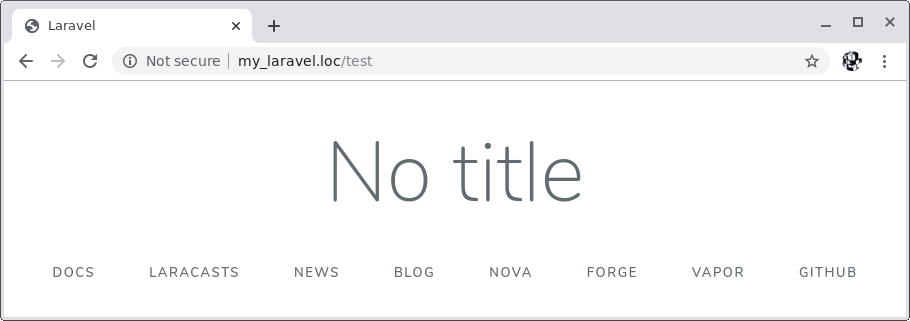
\includegraphics[scale=0.5]{./Pictures/008_blade.png}
\end{figure}

\textbf{routes/web.php}
\begin{minted}{php}
  <?php

  /*
  |--------------------------------------------------------------------------
  | Web Routes
  |--------------------------------------------------------------------------
  |
  | Here is where you can register web routes for your application. These
  | routes are loaded by the RouteServiceProvider within a group which
  | contains the "web" middleware group. Now create something great!
  |
  */

  Route::get('/', function () {
      return view('welcome');
  });

  Route::get('/test', function () {
      return view('test', [
          'title' => 'Curso Laravel en Platzi!!!'
      ]);
  });
\end{minted}

\begin{figure}[h!]
  \centering
  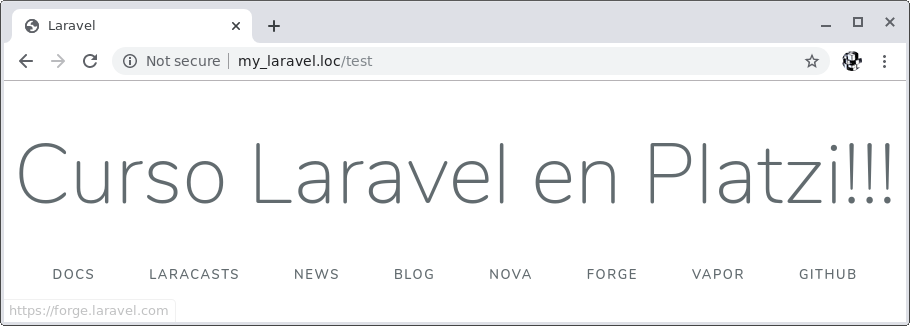
\includegraphics[scale=0.5]{./Pictures/009_blade.png}
\end{figure}

%% Clase 5
\section{Controladores en Laravel}%
Basados en el modelo MVC, vimos que las vistas las tenemos en resources/views,
igualmente en la carpeta app/Http/Controllers podremos definir nuestros
controladores.\\
Aunque podemos utilizar closures directamente dentro de las rutas, Laravel
viene preparado para que trabajemos con controladores.\\

\begin{itemize}
  \item Cuando utilizamos el comando "artisan", encontramos una sección llamada
    "make" que nos va a permitir crear diferentes cosas en el proyecto.
    make:controller nos crea un nuevo controlador.
  \item En nuestro archivo web.php, en la parte de los parámetros, en vez de
    poner un closure vamos a poner el nombre del controlador que creamos
    seguido de una @ y finalizando el método que llamaremos de ese controlador.
\end{itemize}

\begin{minted}{bash}
  php artisan make:controller --help
\end{minted}

\begin{figure}[h!]
  \centering
  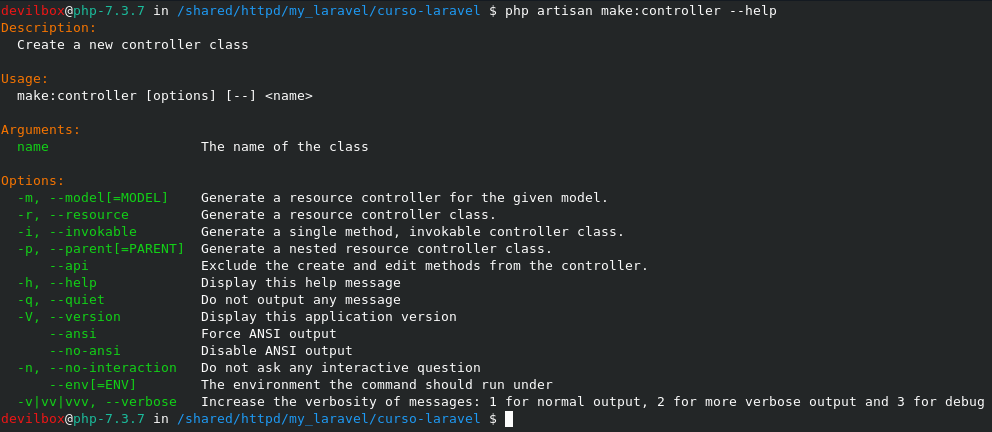
\includegraphics[scale=0.5]{./Pictures/010_artisan_make_controller.png}
\end{figure}

\begin{minted}{bash}
  php artisan make:controller HomeController
\end{minted}

\begin{figure}[h!]
  \centering
  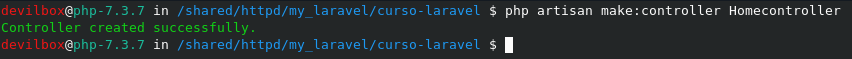
\includegraphics[scale=0.5]{./Pictures/011_artisar_make_controller.png}
\end{figure}

Luego vamos a modificar el HomeController que se ha creado dentro de nuestra
ruta  \textbf{Http/Controllers/HomeController.php}\\

\textbf{Http/Controllers/HomeController.php}
\begin{minted}{php}
  <?php

  namespace App\Http\Controllers;

  use Illuminate\Http\Request;

  class HomeController extends Controller {
      public function index() {
          return view('welcome');
      }
  }
\end{minted}

También modificamos:

\textbf{routes/web.php}
\begin{minted}{php}
  <?php

  /*
  |--------------------------------------------------------------------------
  | Web Routes
  |--------------------------------------------------------------------------
  |
  | Here is where you can register web routes for your application. These
  | routes are loaded by the RouteServiceProvider within a group which
  | contains the "web" middleware group. Now create something great!
  |
  */

  Route::get('/', 'HomeController@index');

  Route::get('/test', function () {
      return view('test', [
          'title' => 'Curso Laravel en Platzi!!!'
      ]);
  });
\end{minted}

\begin{figure}[h!]
  \centering
  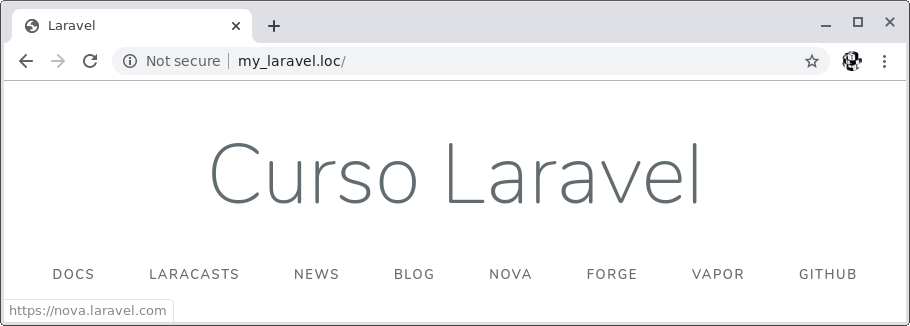
\includegraphics[scale=0.5]{./Pictures/012_homeController.png}
\end{figure}

Ahora crearemos un controller \textbf{DashboardController} ya organizando
nuestro código para el proyecto.\\

\begin{minted}{bash}
  php artisan make:controller DashboardController
\end{minted}

\begin{figure}[h!]
  \centering
  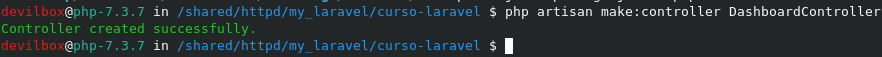
\includegraphics[scale=0.5]{./Pictures/014_dashboardController.png}
\end{figure}

\textbf{app/Http/Controllers/DashboardController.php}
\begin{minted}{java}
  <?php

  namespace App\Http\Controllers;

  use Illuminate\Http\Request;

  class DashboardController extends Controller
  {
      public function index() {
          return view('test', [
              'title' => 'Curso Laravel en Platzi!!!'
          ]);
      }
  }
\end{minted}


\textbf{routes/web.php}
\begin{minted}{java}
  <?php

  /*
  |--------------------------------------------------------------------------
  | Web Routes
  |--------------------------------------------------------------------------
  |
  | Here is where you can register web routes for your application. These
  | routes are loaded by the RouteServiceProvider within a group which
  | contains the "web" middleware group. Now create something great!
  |
  */

  Route::get('/', 'HomeController@index');
  Route::get('/dashboard', 'DashboardController@index');
\end{minted}

\begin{figure}[h!]
  \centering
  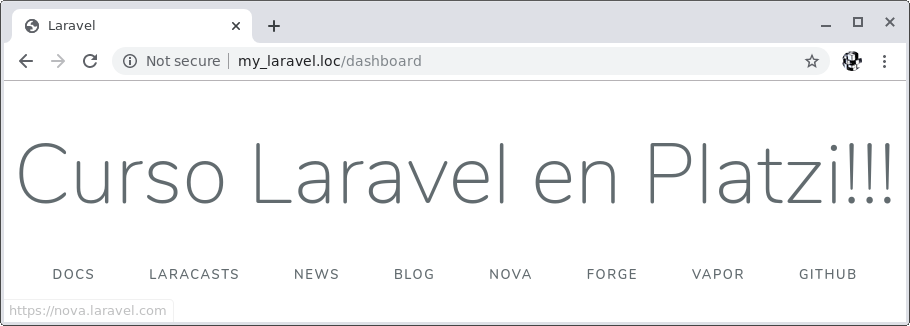
\includegraphics[scale=0.5]{./Pictures/013_dashboardController.png}
\end{figure}



%% Clase 6
\textbf{Request}
El Request es el que contendrá la información que llega cuando alguien hace una
petición al servidor. Se podrán traer parámetros get, datos de formulario en
post o datos en la URL.\\

\begin{itemize}
  \item Laravel utiliza inyección de dependencias y cuando detecta que se
    recibe una variable request, sabe que debe inyectar el request que está
    accediendo a la acción.
  \item Contamos con un helper muy útil de Laravel que reemplaza el var\_dump y
    el die; este helper es dd.
\end{itemize}

\begin{figure}[h!]
  \centering
  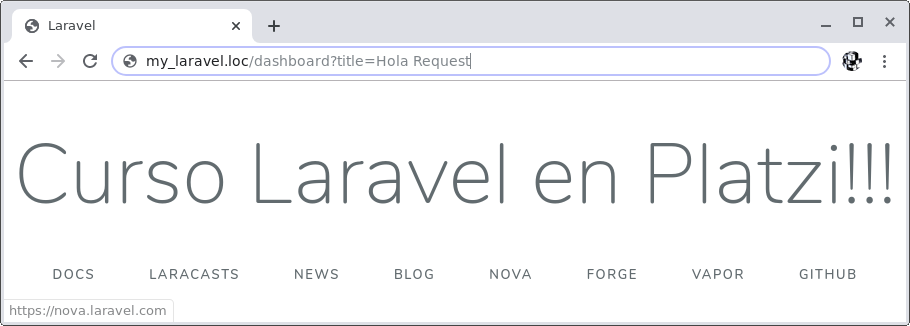
\includegraphics[scale=0.5]{./Pictures/015_request.png}
\end{figure}

\textbf{app/Http/Controllers/DashboardController.php}
\begin{minted}{php}
  <?php

  namespace App\Http\Controllers;

  use Illuminate\Http\Request;

  class DashboardController extends Controller
  {
      public function index(Request $request) {
          var_dump($request); die;
          return view('test', [
              'title' => 'Curso Laravel en Platzi!!!'
          ]);
      }
  }
\end{minted}

\begin{figure}[h!]
  \centering
  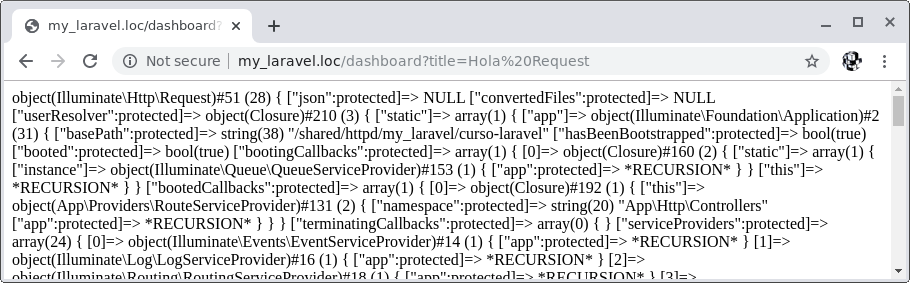
\includegraphics[scale=0.5]{./Pictures/016_vardump_request.png}
\end{figure}

\textbf{app/Http/Controllers/DashboardController.php}
\begin{minted}{php}
  <?php

  namespace App\Http\Controllers;

  use Illuminate\Http\Request;

  class DashboardController extends Controller
  {
      public function index(Request $request) {
          dd($request->query('title'));
          return view('test', [
              'title' => 'Curso Laravel en Platzi!!!'
          ]);
      }
  }
\end{minted}

\begin{figure}[h!]
  \centering
  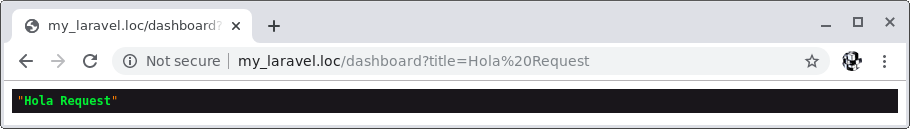
\includegraphics[scale=0.5]{./Pictures/017_dd_title.png}
\end{figure}

\begin{figure}[h!]
  \centering
  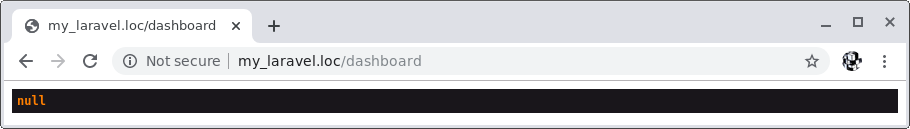
\includegraphics[scale=0.5]{./Pictures/018_dd_title_null.png}
\end{figure}

\textbf{app/Http/Controllers/DashboardController.php}
\begin{minted}{php}
  <?php

  namespace App\Http\Controllers;

  use Illuminate\Http\Request;

  class DashboardController extends Controller
  {
      public function index(Request $request) {
          dd($request->query('title', 'Valor default'));
          return view('test', [
              'title' => 'Curso Laravel en Platzi!!!'
          ]);
      }
  }
\end{minted}

\begin{figure}[h!]
  \centering
  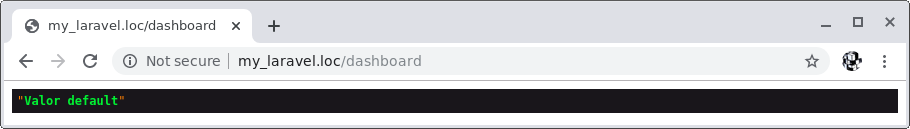
\includegraphics[scale=0.5]{./Pictures/019_dd_title_default.png}
\end{figure}

\textbf{app/Http/Controllers/DashboardController.php}
\begin{minted}{php}
  <?php

  namespace App\Http\Controllers;

  use Illuminate\Http\Request;

  class DashboardController extends Controller
  {
      public function index(Request $request) {
          return view('test', [
              'title' => $request->query('title', 'Valor default')
          ]);
      }
  }
\end{minted}

\begin{figure}[h!]
  \centering
  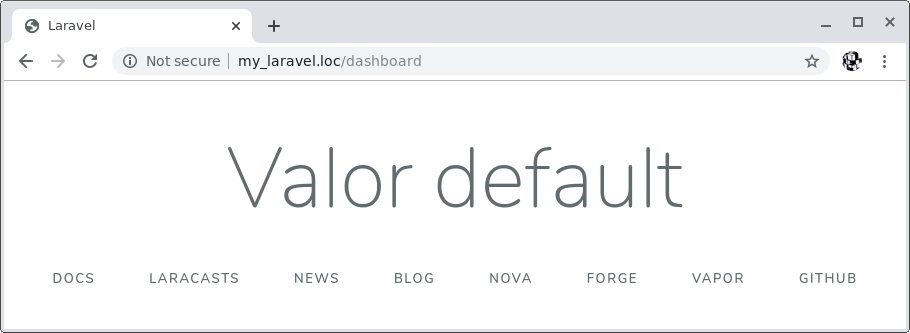
\includegraphics[scale=0.5]{./Pictures/020_title_default.png}
\end{figure}

\begin{figure}[h!]
  \centering
  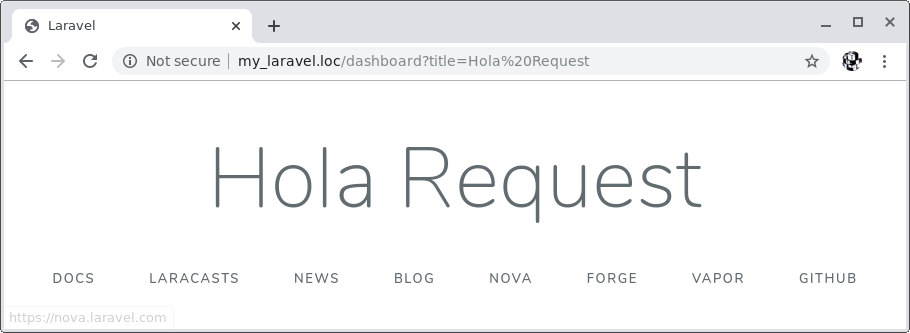
\includegraphics[scale=0.5]{./Pictures/021_title_hola_request.png}
\end{figure}



%% Clase 7
\section{Configuración de laravel}%
En nuestro archivo .env encontraremos mucha información sobre cómo se está
configurando Laravel como el nombre, el entorno de desarrollo, si muestra o no
debug, la URL de nuestra app, datos de conexión a nuestra base de datos, entre
otras opciones.\\

\textbf{APP\_NAME} indica el nombre de la aplicación, \textbf{APP\_ENV} recibe
"local" cuando se está en desarrollo y \textbf{production} es cuando ya lo
liberamos, en \textbf{APP\_DEBUG} especificamos si nuestra aplicación muestra
los errores o no los muestra, en \textbf{DB\_CONNECTION} indica la base de datos
en la que estás trabajando (recuerda que Laravel trabaja con un ORM llamado
Eloquent), \textbf{DB\_HOST} almacena la dirección del host, \textbf{DB\_PORT} el
puerto, \textbf{DB\_DATABASE} el nombre de la base de datos,
\textbf{DB\_USERNAME} el nombre de usuario, \textbf{DB\_PASSWORD} la
contraseña.\\

Para este ejemplo vamos a utilizar como nombre de nuestra base de datos
\textbf{cursolaravel} y en  \textbf{DB\_HOST} ya que estamos trabajando en
devilbox entonces indicaremos el virtualhost creado, en nuestro caso se llama
\textbf{my\_laravel.loc}\\

Veamos el contenido de \textbf{.env} con los cambios realizados:

\textbf{.env}
\begin{minted}{php}
  APP_NAME=Laravel
  APP_ENV=local
  APP_KEY=base64:CuYUhd6VUrFS1OrNbVb4TzqjGEQqkCcMIUQfjJKK0dI=
  APP_DEBUG=true
  APP_URL=http://localhost

  LOG_CHANNEL=stack

  DB_CONNECTION=mysql
  DB_HOST=my_laravel.loc
  DB_PORT=3306
  DB_DATABASE=cursolaravel
  DB_USERNAME=root
  DB_PASSWORD=

  BROADCAST_DRIVER=log
  CACHE_DRIVER=file
  QUEUE_CONNECTION=sync
  SESSION_DRIVER=file
  SESSION_LIFETIME=120

  REDIS_HOST=127.0.0.1
  REDIS_PASSWORD=null
  REDIS_PORT=6379

  MAIL_DRIVER=smtp
  MAIL_HOST=smtp.mailtrap.io
  MAIL_PORT=2525
  MAIL_USERNAME=null
  MAIL_PASSWORD=null
  MAIL_ENCRYPTION=null

  AWS_ACCESS_KEY_ID=
  AWS_SECRET_ACCESS_KEY=
  AWS_DEFAULT_REGION=us-east-1
  AWS_BUCKET=

  PUSHER_APP_ID=
  PUSHER_APP_KEY=
  PUSHER_APP_SECRET=
  PUSHER_APP_CLUSTER=mt1

  MIX_PUSHER_APP_KEY="${PUSHER_APP_KEY}"
  MIX_PUSHER_APP_CLUSTER="${PUSHER_APP_CLUSTER}"
\end{minted}


Toda la configuración que hacemos realmente se está llamando dentro de los
archivos que están en la carpeta config\\

Ahora vamos a crear una nueva base de datos:

\begin{itemize}
  \item Si vienes del curso de introducción a PHP, seguramente tienes
    PHPMyAdmin el cual puedes seguir usando o puedes cambiar a cualquier
    cliente que te guste.
\end{itemize}

\begin{figure}[h!]
  \centering
  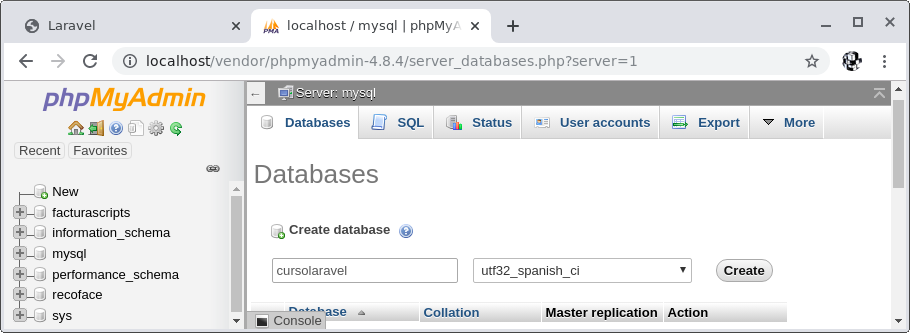
\includegraphics[scale=0.5]{./Pictures/022_bd.png}
\end{figure}


%% Clase 8
\section{Cómo funcionan las Migraciones de DB}%
Laravel ofrece un sistema de migraciones de bases de datos las cuales pueden
ser vistas como una especie de control de código pero para bases de datos. Esto
es muy útil para equipos de trabajo al poder tener los cambios en el
repositorio y de esta manera cada miembro del equipo podrá ejecutar las
migraciones para tener los esquemas adecuados.\\

\begin{itemize}
  \item Tenemos un comando llamado make:migration que nos permite generar
    archivos de migraciones.
  \item Contamos con una sección entera llamada migrate que nos servirá para
    realizar diferentes acciones relacionadas con las migraciones. Si
    ejecutamos migrate sin nada más, ejecutará todas las migraciones pendientes
    en el equipo.
  \item migrate:fresh va a borrar todas las tablas y las creará de nuevo
    utilizando todas las migraciones que tenemos.
  \item migrate:rollback nos permite regresar un paso.
\end{itemize}

Puedes encontrar las migraciones en la carpeta database/migrations. Laravel nos
ofrece tres migraciones de inicio que son para crear tablas de usuarios, para
crear una tabla de resets de passwords y otra tabla para registrar trabajos
fallidos.\\

\begin{minted}{bash}
  php artisan migrate
\end{minted}

\begin{figure}[h!]
  \centering
  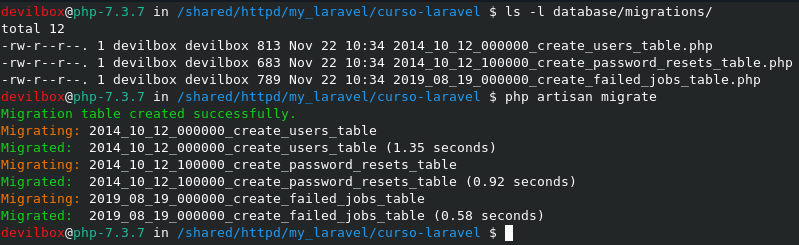
\includegraphics[scale=0.5]{./Pictures/023_migrate.png}
\end{figure}

\begin{figure}[h!]
  \centering
  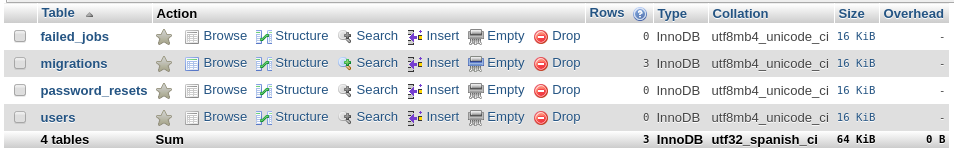
\includegraphics[scale=0.5]{./Pictures/024_migrate.png}
\end{figure}

Si vemos el contenido de la tabla migrations, encontraremos los ficheros que se
encontraban en database/migrations, si en caso nosotros añadimos algun fichero
entonces este no figurará en esta tabla hasta que hagamos la migración.\\

\begin{figure}[h!]
  \centering
  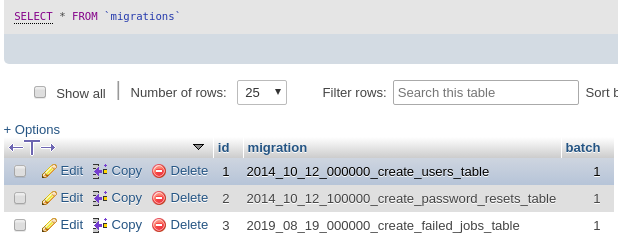
\includegraphics[scale=0.5]{./Pictures/025_table_migrations.png}
\end{figure}


Las migraciones tienen dos partes:

\begin{itemize}
  \item up, que nos dice qué va a crear la migración.
  \item down, que revierte lo que se hizo en la migración, activado al hacer
    rollback.
\end{itemize}

Al correr las migraciones se nos crearán 3 tablas, una de ella siendo
migrations que nos llevará el control de cómo se va generando cada cambio.\\

Laravel nos ofrece Schema que nos trae diferentes cosas para trabajar sobre los
sistemas de bases de datos.\\


%% Clase 9
\section{Migraciones en Artisan}%
Laravel es un framework de código abierto que agiliza el desarrollo de
aplicaciones web con PHP utilizando la arquitectura MVC y nos permite resolver
necesidades actuales como el manejo de eventos y la autenticación de usuarios.
Además, cuenta con un código modular y extensible por medio de un administrador
de paquetes y un soporte robusto para manejo de bases de datos.\\


\begin{minted}{bash}
  php artisan make:migration create_table_expense_reports --create=expense_reports
\end{minted}

\begin{figure}[h!]
  \centering
  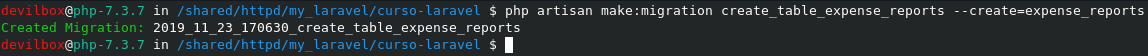
\includegraphics[scale=0.5]{./Pictures/026_create_table_artisan.png}
\end{figure}

\begin{figure}[h!]
  \centering
  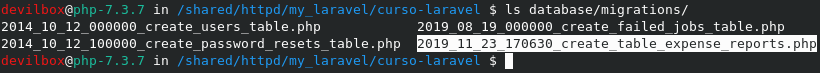
\includegraphics[scale=0.5]{./Pictures/027_migration_file.png}
\end{figure}


\begin{minted}{bash}
  php artisan migrate
\end{minted}

\begin{figure}[h!]
  \centering
  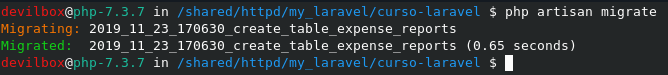
\includegraphics[scale=0.5]{./Pictures/028_migrate.png}
\end{figure}

Luego vemos que se ha creado la tabla correctamente, con algunos campos
predeterminados.\\

\begin{figure}[h!]
  \centering
  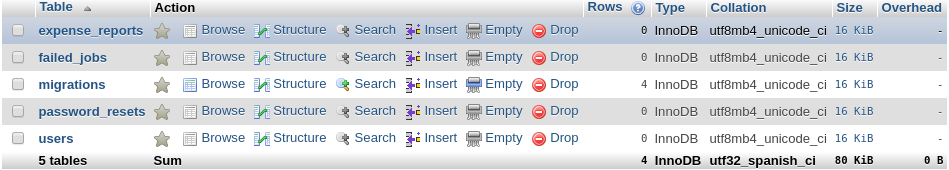
\includegraphics[scale=0.5]{./Pictures/029_table_created.png}
\end{figure}

\begin{figure}[h!]
  \centering
  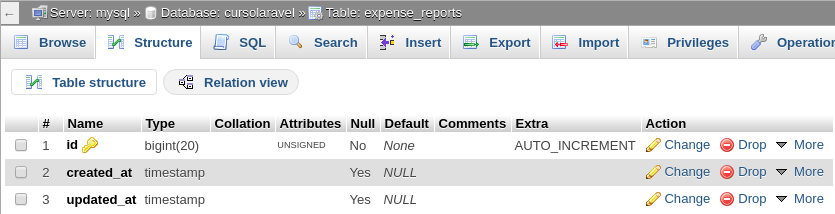
\includegraphics[scale=0.5]{./Pictures/030_expense_reports.png}
\end{figure}

Como se observa ahora se ha agregado el nombre del fichero a la tabla
migrations.

\begin{figure}[h!]
  \centering
  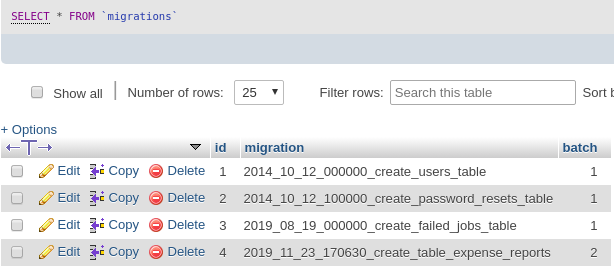
\includegraphics[scale=0.5]{./Pictures/031_migrations_table.png}
\end{figure}

Nótece los números que se encuentran en el campo \textbf{batch}.\\
Estos números nos sirven de guía cuando hagamos \textbf{rollback}.

\begin{minted}{bash}
  php artisan migrate:rollback
\end{minted}

\begin{figure}[h!]
  \centering
  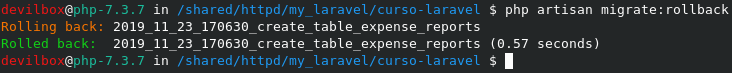
\includegraphics[scale=0.5]{./Pictures/032_rollback.png}
\end{figure}

Veamos la tabla \textbf{migrations} esta vez.

\begin{figure}[h!]
  \centering
  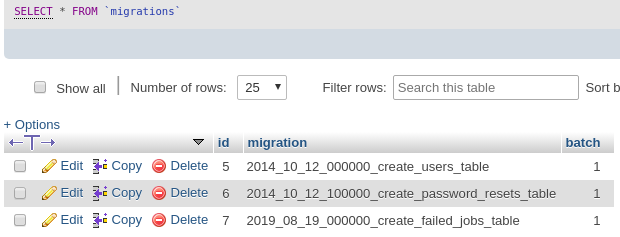
\includegraphics[scale=0.5]{./Pictures/033_migrations_table.png}
\end{figure}

Si hacemos nuevamente un \textbf{rollback}.

\begin{figure}[h!]
  \centering
  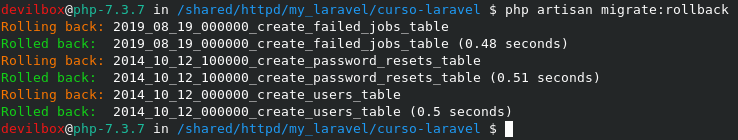
\includegraphics[scale=0.5]{./Pictures/034_rolback.png}
\end{figure}

Como observamos ahora, no hay ningun registro en nuestra tabla
\textbf{migrations}.

\begin{figure}[h!]
  \centering
  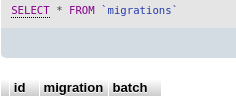
\includegraphics[scale=0.5]{./Pictures/035_migrations_table.png}
\end{figure}

Sin embargo los archivos de migración aún se encuentran en nuestro directorio
\textbf{database/migrations}.\\
Podemos usar el siguiente comando para reestableces nuestras tablas.\\

\begin{minted}{bash}
  php artisan migrate
\end{minted}

\begin{figure}[h!]
  \centering
  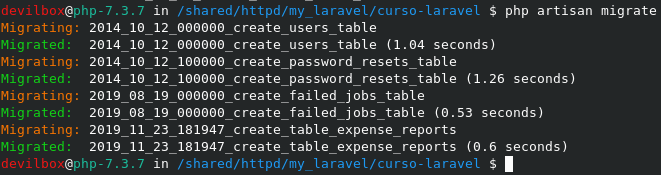
\includegraphics[scale=0.5]{./Pictures/036_migrate_again.png}
\end{figure}

\begin{figure}[h!]
  \centering
  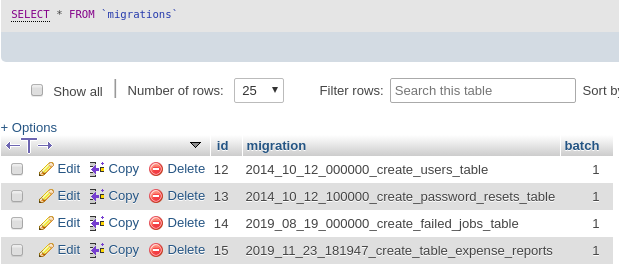
\includegraphics[scale=0.5]{./Pictures/037_migrations_table.png}
\end{figure}

Como se observa, ahora todos los registros en nuestra tabla \textbf{migrations}
tienen \textbf{batch} con valor 1.


%% Clase 10
\section{Modelos con Eloquent}%
Un ORM es un sistema que nos permite mapear registros de la base de datos a
objetos dentro dentro de nuestro código. No es exclusivo de PHP ya que se usa
mucho en los lenguajes de programación orientada a objetos.\\

\begin{itemize}
  \item make:model crea una nueva clase para representar un modelo de Eloquent.
  \item Cuando creamos las bases de datos es estándar que las tablas tengan el
    nombre en plural pero los modelos como representan una clase que representa
    un objeto, tendrán su nombre en singular.
  \item Todos los modelos los podremos encontrar dentro de la carpeta app.
    Laravel no tiene carpeta models porque los creadores creen que model puede
    tener muchos significados.
  \item El comando tinker nos ofrece un entorno de pruebas para ver cómo
    funcionan las cosas que estamos haciendo. Tiene en cuenta variables de
    entorno, lo que inicializa Laravel y también sabe que estamos usando
    Eloquent.
\end{itemize}

Siempre podemos visualizar información de ayuda para el uso de los comandos
agregando el flag --help.

\begin{minted}{bash}
  php artisan make:model --help
\end{minted}

\begin{figure}[h!]
  \centering
  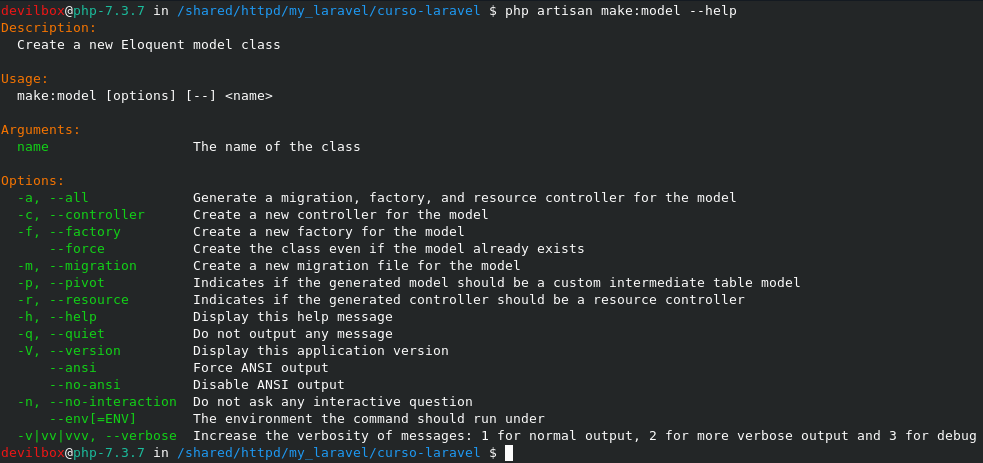
\includegraphics[scale=0.5]{./Pictures/038_make_model_help.png}
\end{figure}

Ahora vamos a crear un Modelo.

\begin{minted}{bash}
  php artisan make:model ExpenseReport
\end{minted}

\begin{figure}[h!]
  \centering
  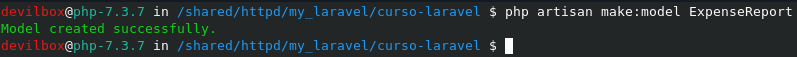
\includegraphics[scale=0.5]{./Pictures/039_model_created.png}
\end{figure}

Con Laravel no hay una carpeta \textbf{Model} o \textbf{Entity}, sino que todos
los modelos se almacenan dentro de la carpeta \textbf{app/}.

\begin{figure}[h!]
  \centering
  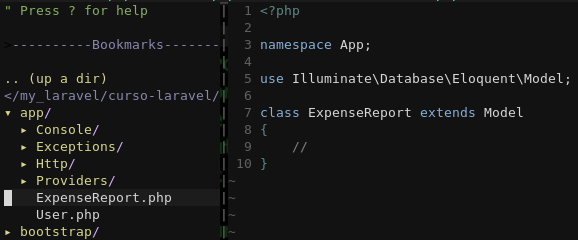
\includegraphics[scale=0.5]{./Pictures/039_model_created_tree.png}
\end{figure}

Hay una herramienta que nos permite interactuar con nuestro código, como una
expecie de entorno de pruebas o sandbox y carga todos los componentes
inicializados que estan incluidos en Laravel, en este caso usaremos Eloquent y
vamos a jugar un poco.\\

\begin{figure}[h!]
  \centering
  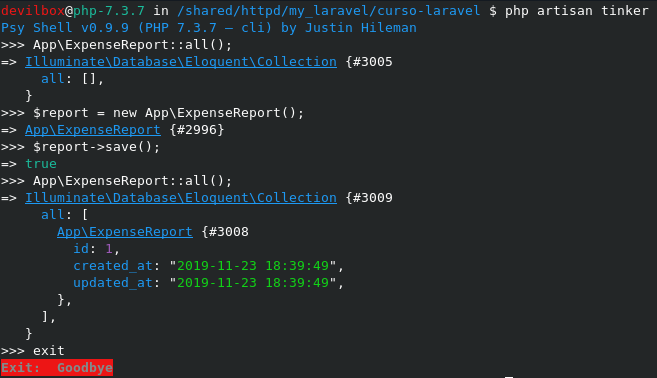
\includegraphics[scale=0.5]{./Pictures/040_artisan_tinker.png}
\end{figure}

Como se ve con la primera instrucción le consultamos cuantos ExpertReports
tenemos actualmente y nos devolvió una colección de Eloquent pero como un array
vacío. En la segunda instrucción creamos un nuevo reporte y nos devuelve que se
creó el reporte, pero es un objeto en memoria. Con la tercera instrucción
persistimos el reporte con el metodo \textbf{save}, esto nos devuelve un true
que indica que se realizó exitosamente. Con la cuarta instrucción volvemos a
consultar el contenido de la tabla con el modelo ExpenseReport y nos devuelve
una colección de eloquent con la propiedad all con el primer ExpenseReport
creado con el id 1 y las fechas de created\_at y updated\_at. Esto lo podemos
visualizar también en nuestro cliente de Base de Datos.\\

\begin{figure}[h!]
  \centering
  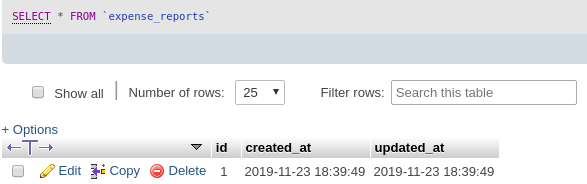
\includegraphics[scale=0.5]{./Pictures/041_registro_expense_reports.png}
\end{figure}


%% Clase 11
\section{Trabajando con un Modelo}%
\begin{itemize}
  \item No es aconsejable modificar una migración ya que si estamos trabajando
    en equipo alguien puede haber ya corrido la migración con anterioridad y
    esto le causaría conflictos. Lo aconsejable es crear una migración
    adicional.
  \item El comando migrate:fresh lo reinicia todo incluyendo la base de datos y
    los elementos creados.
\end{itemize}

Para crear una migration entonces lo hacemos usando artisan indicando el nombre
de la tabla.
\begin{minted}{bash}
  php artisan make:migration create_column_title_in_reports --table=expense_reports
\end{minted}

\begin{figure}[h!]
  \centering
  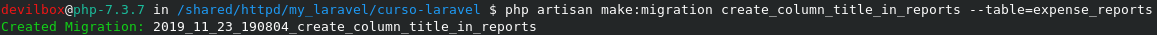
\includegraphics[scale=0.5]{./Pictures/040_migration_file.png}
\end{figure}

\begin{figure}[h!]
  \centering
  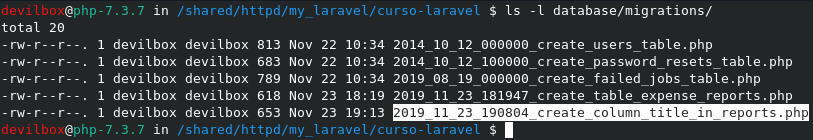
\includegraphics[scale=0.5]{./Pictures/042_php_migration.png}
\end{figure}

\textbf{database/migrations/2019\_11\_23\_190804\_create\_column\_title\_in\_reports.php}
\begin{minted}{php}
  <?php

  use Illuminate\Database\Migrations\Migration;
  use Illuminate\Database\Schema\Blueprint;
  use Illuminate\Support\Facades\Schema;

  class CreateColumnTitleInReports extends Migration
  {
      /**
      * Run the migrations.
      *
      * @return void
      */
      public function up()
      {
          Schema::table('expense_reports', function (Blueprint $table) {
              $table->text('title');
          });
      }

      /**
      * Reverse the migrations.
      *
      * @return void
      */
      public function down()
      {
          Schema::table('expense_reports', function (Blueprint $table) {
              $table->dropColumn('title');
          });
      }
  }
\end{minted}

Luego hacemos la migración:
\begin{minted}{bash}
  php artisan migrate
\end{minted}

\begin{figure}[h!]
  \centering
  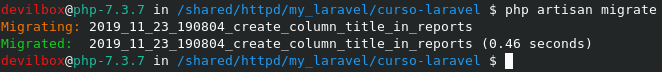
\includegraphics[scale=0.5]{./Pictures/041_migrate.png}
\end{figure}

Luego revisamos la tabla y verificamos que se ha creado el campo
\textbf{title} de tipo text.\\

\begin{figure}[h!]
  \centering
  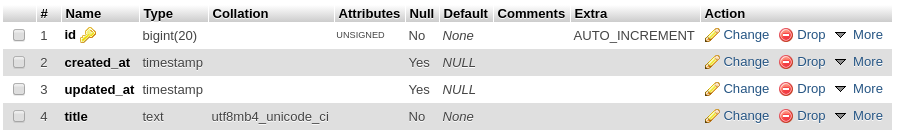
\includegraphics[scale=0.5]{./Pictures/043_title.png}
\end{figure}

También revisemos el contenido de la tabla \textbf{migrations} y observamos que
se creó un nuevo registro con el nombre de nuestro fichero de migración y con
el campo \textbf{batch} en valor 2.\\

Por último con \textbf{fresh} podemos eliminar todo el contenido de nuestras
bases de datos y crear nuevamente las tablas.

\begin{minted}{bash}
  php artisan migrate:fresh
\end{minted}

\begin{figure}[h!]
  \centering
  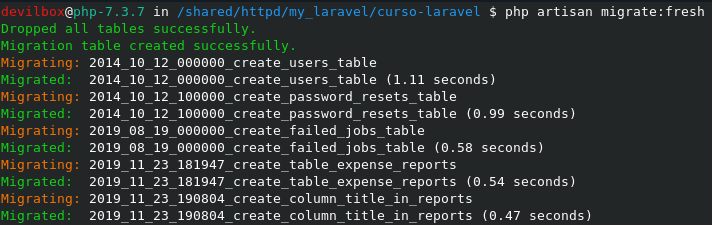
\includegraphics[scale=0.5]{./Pictures/044_migrate_fresh.png}
\end{figure}

\begin{figure}[h!]
  \centering
  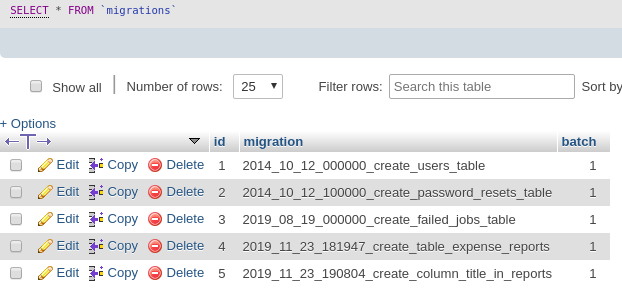
\includegraphics[scale=0.5]{./Pictures/045_migration_fresh.png}
\end{figure}

Como vemos la tabla \textbf{migrations} ahora tiene todos los registros con el
\textbf{batch} en valor 1. Además el registro que teníamos en la tabla
\textbf{expense\_reports} también ha desaparecido.\\

\begin{figure}[h!]
  \centering
  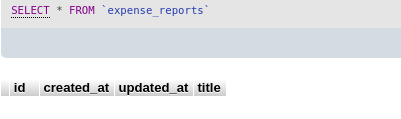
\includegraphics[scale=0.5]{./Pictures/046_expense_report_dropped.png}
\end{figure}

Entonces vamos usar \textbf{tinker} para crear un registro en la tabla.

\begin{minted}{bash}
  php artisan tinker
\end{minted}

\begin{figure}[h!]
  \centering
  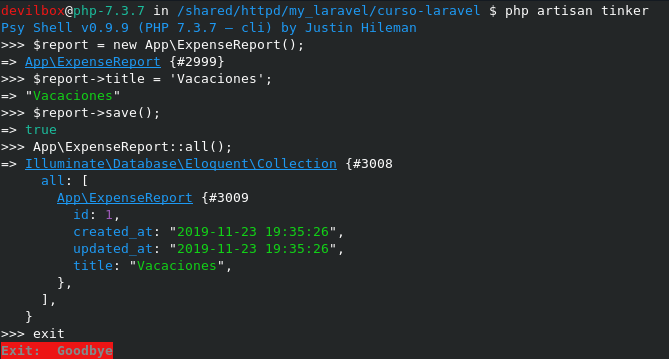
\includegraphics[scale=0.5]{./Pictures/047_new_reg_tinker.png}
\end{figure}

También podemos visualizar el registro en nuestro cliente de Base de Datos.

\begin{figure}[h!]
  \centering
  \includegraphics[scale=0.5]{./Pictures/048_expense_report.png}
\end{figure}


%% Clase 12
\section{Controladores y recursos}%
CRUD significa create (crear), read (leer), update (actualizar o editar),
delete (eliminar).\\

\textbf{resource} genera una clase de controlador de tipo recurso. Esto
significa que tendremos todo lo necesario para poder hacer CRUD.\\

\begin{itemize}
  \item index: Aquí se despliegan todos los elementos a mostrar.
  \item create: Creará nuevos elementos.
  \item store: Guardará los elementos creados en create.
  \item show: Mostrará a detalle un solo elemento y por eso es que recibe un id.
  \item edit: Edita los elementos que mostramos en show.
  \item update: Almacena los cambios de edit en la base de datos.
  \item destroy: Eliminará los elementos.
\end{itemize}

Creamos nuestro controller con el flag \textbf{--resource}. Esto nos creará los
métodos en blanco para poder realizar CRUD con nuestro controller.\\

\begin{minted}{bash}
  php artisan make:controller ExpenseReportController --resource
\end{minted}

\begin{figure}[h!]
  \centering
  \includegraphics[scale=0.5]{./Pictures/049_controller_resource.png}
\end{figure}

En route:list podremos ver todas las rutas que tenemos definidas\\

\begin{figure}[h!]
  \centering
  \includegraphics[scale=0.5]{./Pictures/050_route_list.png}
\end{figure}

Para crear una ruta de un controlador resource no usamos get o post, sino
directamente la estructura Route::resource(); ya que de esta manera se nos
crearán rutas para cada uno de los métodos anteriormente mencionados que son
creados por el controlador resource.

\textbf{routes/web.php}
\begin{minted}{php}
  <?php

  /*
  |--------------------------------------------------------------------------
  | Web Routes
  |--------------------------------------------------------------------------
  |
  | Here is where you can register web routes for your application. These
  | routes are loaded by the RouteServiceProvider within a group which
  | contains the "web" middleware group. Now create something great!
  |
  */

  Route::get('/', 'HomeController@index');
  Route::get('/dashboard', 'DashboardController@index');
  Route::resource('/expense_reports', 'ExpenseReportController');
\end{minted}

Con solo hacer esto, veamos nuevamente la lista de nuestras rutas.

\begin{minted}{bash}
  php artisan route:list
\end{minted}

\begin{figure}[h!]
  \centering
  \includegraphics[scale=0.5]{./Pictures/051_rout_list_after.png}
\end{figure}

Ahora vamos a modificar el método index dentro de ExpenseReportController para
mostrar todos los registros que tenga.

\textbf{app/Http/Controllers/}
\begin{minted}{php}
  <?php

  namespace App\Http\Controllers;

  use App\ExpenseReport;
  use Illuminate\Http\Request;

  class ExpenseReportController extends Controller
  {
      /**
      * Display a listing of the resource.
      *
      * @return \Illuminate\Http\Response
      */
      public function index()
      {
          return ExpenseReport::all();
      }

      /**
      * Show the form for creating a new resource.
      *
      * @return \Illuminate\Http\Response
      */
      public function create()
      {
          //
      }

      /**
      * Store a newly created resource in storage.
      *
      * @param  \Illuminate\Http\Request  $request
      * @return \Illuminate\Http\Response
      */
      public function store(Request $request)
      {
          //
      }

      /**
      * Display the specified resource.
      *
      * @param  int  $id
      * @return \Illuminate\Http\Response
      */
      public function show($id)
      {
          //
      }

      /**
      * Show the form for editing the specified resource.
      *
      * @param  int  $id
      * @return \Illuminate\Http\Response
      */
      public function edit($id)
      {
          //
      }

      /**
      * Update the specified resource in storage.
      *
      * @param  \Illuminate\Http\Request  $request
      * @param  int  $id
      * @return \Illuminate\Http\Response
      */
      public function update(Request $request, $id)
      {
          //
      }

      /**
      * Remove the specified resource from storage.
      *
      * @param  int  $id
      * @return \Illuminate\Http\Response
      */
      public function destroy($id)
      {
          //
      }
  }
\end{minted}

Luego vamos a nuestro navegador y escribimos en el url /expense\_reports\\

\begin{figure}[h!]
  \centering
  \includegraphics[scale=0.5]{./Pictures/052_expense_reports.png}
\end{figure}

Ahora vamos a añadirle una vista. Para esto vamos a copiar el contenido de la
vista \textbf{welcome.blade.php} en una nueva carpeta llamada
\textbf{expenseReport}, con la finalidad de ir organizando nuestras vistas en
el fichero llamado \textbf{index.blade.php}.\\

Luego vamos a modificar el contenido de la siguiente manera:

\textbf{resources/views/expenseReport/index.blade.php}
\begin{minted}{html+php}
  <!DOCTYPE html>
  <html lang="{{ str_replace('_', '-', app()->getLocale()) }}">
      <head>
          <meta charset="utf-8">
          <meta name="viewport" content="width=device-width, initial-scale=1">

          <title>Laravel</title>

          <!-- Fonts -->
          <link href="https://fonts.googleapis.com/css?family=Nunito:200,600" rel="stylesheet">

          <!-- Styles -->
          <style>
              html, body {
                  background-color: #fff;
                  color: #636b6f;
                  font-family: 'Nunito', sans-serif;
                  font-weight: 200;
                  height: 100vh;
                  margin: 0;
              }

              .full-height {
                  height: 100vh;
              }

              .flex-center {
                  align-items: center;
                  display: flex;
                  justify-content: center;
              }

              .position-ref {
                  position: relative;
              }

              .top-right {
                  position: absolute;
                  right: 10px;
                  top: 18px;
              }

              .content {
                  text-align: center;
              }

              .title {
                  font-size: 84px;
              }

              .links > a {
                  color: #636b6f;
                  padding: 0 25px;
                  font-size: 13px;
                  font-weight: 600;
                  letter-spacing: .1rem;
                  text-decoration: none;
                  text-transform: uppercase;
              }

              .m-b-md {
                  margin-bottom: 30px;
              }
          </style>
      </head>
      <body>
          <div class="flex-center position-ref full-height">
              @if (Route::has('login'))
                  <div class="top-right links">
                      @auth
                          <a href="{{ url('/home') }}">Home</a>
                      @else
                          <a href="{{ route('login') }}">Login</a>

                          @if (Route::has('register'))
                              <a href="{{ route('register') }}">Register</a>
                          @endif
                      @endauth
                  </div>
              @endif

              <div class="content">
                  <div class="row">
                      <div class="col">
                          <h1>Reports</h1>
                          <table class="table">
                              @foreach ($expenseReports as $expenseReport)
                                  <tr>
                                      <td>{{ $expenseReport->title }}</td>
                                  </tr>
                              @endforeach
                          </table>
                      </div>
                  </div>
              </div>
          </div>
      </body>
  </html>
\end{minted}

Actualizamos en nuestro navegador y obtenemos:\\

\begin{figure}[h!]
  \centering
  \includegraphics[scale=0.5]{./Pictures/053_expense_reports_ok.png}
\end{figure}



%% Clase 13
\section{Blade layout}%
Cuando se tienen muchas vistas que repiten gran parte del código HTML, una
mejor práctica para evitar esta repetición es crear layouts y extender de
ellos. De esta manera el layout tendrá el contenido que siempre se repite y los
hijos el código específico de ellos.\\

\begin{itemize}
  \item @yield marca la parte en donde irá el código de los hijos que extiendan
    o hereden del layout.
  \item En las vistas hijas se utiliza @section para decir que esa parte del
    código es la que concuerda con el @yield del layout.
\end{itemize}

Veamos en el proyecto. Creamos una carpeta dentro de \textbf{resources/views}
llamada \textbf{layouts} donde agregaremos el starter template de bootstrap que
podemos encontrar al principio de su documentación en la siguiente
\href{https://getbootstrap.com/docs/4.3/getting-started/introduction/}{página}
en el archivo \textbf{base.blade.php}.\\

\textbf{resouces/views/layouts/base.blade.php}
\begin{minted}{html+php}
  <!doctype html>
  <html lang="en">
    <head>
      <!-- Required meta tags -->
      <meta charset="utf-8">
      <meta name="viewport" content="width=device-width, initial-scale=1,
                  shrink-to-fit=no">

      <!-- Bootstrap CSS -->
      <link rel="stylesheet"
            href="https://stackpath.bootstrapcdn.com/bootstrap/4.3.1/css/bootstrap.min.css"
            integrity="sha384-ggOyR0iXCbMQv3Xipma34MD+dH/1fQ784/j6cY/iJTQUOhcWr7x9JvoRxT2MZw1T"
            crossorigin="anonymous">

      <title>Expense Reports</title>
    </head>
    <body>
      <div class="container">
        @yield('content')
      </div>

      <!-- Optional JavaScript -->
      <!-- jQuery first, then Popper.js, then Bootstrap JS -->
      <script src="https://code.jquery.com/jquery-3.3.1.slim.min.js"
              integrity="sha384-q8i/X+965DzO0rT7abK41JStQIAqVgRVzpbzo5smXKp4YfRvH+8abtTE1Pi6jizo"
              crossorigin="anonymous"></script>
      <script
        src="https://cdnjs.cloudflare.com/ajax/libs/popper.js/1.14.7/umd/popper.min.js"
        integrity="sha384-UO2eT0CpHqdSJQ6hJty5KVphtPhzWj9WO1clHTMGa3JDZwrnQq4sF86dIHNDz0W1"
        crossorigin="anonymous"></script>
      <script
        src="https://stackpath.bootstrapcdn.com/bootstrap/4.3.1/js/bootstrap.min.js"
        integrity="sha384-JjSmVgyd0p3pXB1rRibZUAYoIIy6OrQ6VrjIEaFf/nJGzIxFDsf4x0xIM+B07jRM"
        crossorigin="anonymous"></script>
    </body>
  </html>
\end{minted}

Luego modificamos el fichero \textbf{index.blade.php} ubicado en el directorio
\textbf{expenseReport}. Borramos todo lo que se repite en el layout y
extendemos de \textbf{layouts/base.blade.php}\\

\textbf{resources/views/expenseReport/index.blade.php}
\begin{minted}{php}
  @extends('layouts.base')

  @section('content')
      <div class="row">
          <div class="col">
              <h1>Reports</h1>
              <table class="table">
                  @foreach ($expenseReports as $expenseReport)
                      <tr>
                          <td>{{ $expenseReport->title }}</td>
                      </tr>
                  @endforeach
              </table>
          </div>
      </div>
  @endsection
\end{minted}

\begin{figure}[h!]
  \centering
  \includegraphics[scale=0.5]{./Pictures/054_extends_layout.png}
\end{figure}



%% Clase 14
\section{Form para agregar reportes}%

%% Clase 15
\section{CSRF}%
CSRF (Cross-site request forgery) es un tipo de ataque que consiste en que un
usuario puede intentar hacer muchas peticiones en nombre de otro. Para esto
Laravel genera con cada sesión un token que se usará para validar que exista el
usuario en el sistema y que sea él quien está haciendo la petición. Esto
también implica que no se pueden hacer peticiones desde otra app hacia el post,
debe manejarse de manera interna.\\

Si queremos que un form pueda pasar la seguridad CSRF de Laravel, debemos
agregar el helper @csrf el cual nos agrega un token.\\

\begin{itemize}
  \item Cuando estamos guardando nuevas entradas en la base de datos podemos
    redireccionar adonde queramos en nuestra aplicación con una respuesta
    especial de Laravel llamada redirect.
\end{itemize}

Estamos trabajando con Middlewares los cuales son muy usados en aplicaciones
web que consisten en capas que contienen el request. Cuando llega un request,
éste deberá pasar por diferentes capas o filtros (middlewares) quienes al final
regresarán una respuesta. Cada uno de los filtros puede detener las peticiones
en caso de que algo no cumpla.\\

Si no se desea usar la protección CSRF se puede directamente quitar el
middleware desde el archivo kernel.php. De la misma manera se pueden crear
middleware propios y agregarlos aquí.\\

%% Clase 16
\section{Fake PUT/PATCH}%
En Laravel cuando usamos recursos nos pone Put y Patch como una opción para
modificar nuestros recursos. El problema de esto es que en un form no se puede
especificar directamente que queremos hacer un Put o un Patch y por esto
Laravel nos ofrece un mecanismo para hacer ”Fake PUT/PATCH” y podamos recibir y
procesar los datos.\\

Para que Laravel acepte el Put o Patch es necesario poner dentro del form de
manera auxiliar @method(‘tipo de método usado’) y así aunque el form tenga un
POST como método, realmente será traducido al que especifiquemos dentro del
auxiliar.\\


%% Clase 17
\section{Borrando reportes}%
De la misma forma en la que pudimos crear un “Fake PUT/PATCH” también podemos
crear una especie de “Fake DELETE”.\\

\begin{itemize}
  \item Con Javascript podemos mostrar una alerta al borrar una entrada que nos
    permita confirmar si la vamos a borrar o no.
  \item Es bueno que las vistas hagan match con la acción porque permite
    encontrar rápidamente qué vista le pertenece a qué acción.
  \item Laravel nos ofrece el helper @method(‘delete’) ya que no se puede
    especificar directamente en el form.
  \item Tenemos con Laravel un método especial findOrFail que permitirá
    regresar un error 404 si un usuario está haciendo algo no válido al
    consultar o editar un registro en la base de datos.
\end{itemize}

%% Clase 18
\section{Validaciones}%
Es muy importante validar siempre la información que los usuarios ingresan en
el sistema. En la mayoría de los casos tendrás usuarios bien intencionados que
sólo busquen hacer uso del sistema, pero puede ocurrir que haya algún atacante
que quiera obtener información que no le pertenece.\\

Cuando por ejemplo se hace submit a un form vacío, no vamos a querer que el
usuario final vea los errores como son lanzados sino manejarlos de alguna
manera, así que los validamos con ayuda de Laravel.\\

Laravel incluye todos los errores de validación que podamos encontrar dentro de
un objeto especial llamado errors el cual podemos usar en nuestro template.\\

\begin{itemize}
  \item Se utiliza la línea vertical | para agregar más validaciones.
  \item Si un usuario se equivoca al llenar los campos de formulario y al
    intentarlo de nuevo debe ingresarlos todos otra vez, eso significará una
    mala experiencia de usuario y creará frustración. Por esto mismo se deben
    poner de nuevo los valores y para esto Laravel nos ofrece un auxiliar
    especial llamado old que podemos usar en el valor del campo.
\end{itemize}


%% Clase 19
\section{Creamos la vista de reportes}%
\begin{itemize}
  \item El método show despliega la información específica para un recurso
    dado.
  \item Existe una técnica en Laravel llamada model binding que antes de llegar
    a la acción realiza el findOrFail y nos envía el objeto que se requiere.
\end{itemize}

%% Clase 20
\section{Relaciones con eloquent}%
\begin{itemize}
  \item Si estamos hablando de un blogpost, es posible que éste esté
    relacionado con múltiples comentarios y a su vez con un solo creador.
    Existen muchas maneras para relacionar bases de datos y esto nos ayudará a
    tener una integridad y una referencia hacia lo que necesitamos.
  \item -m o –migration son exactamente lo mismo y se pueden usar
    indistintamente.
  \item Haremos una relación de muchos a uno, es decir que un reporte puede
    tener muchos detalles.
  \item PHP en sus últimas versiones nos ofrece que todas las clases contienen
    la propiedad estática que es el nombre de la clase y la regresa
    directamente.
\end{itemize}


%% Clase 21
\section{Trabajando con relaciones}%
Comenzaremos a usar tablas relacionadas


%% Clase 22
\section{Acción para enviar un mail}%
Siguiendo el proyecto que se viene trabajando en el curso, y también en muchos
otros proyectos que realices puedes querer implementar un sistema de envío de
mails por diferentes motivos, sea avisar a alguien de tu empresa que deba salir
de viaje sobre algo que esté sucediendo o avisar a tus clientes de alguna
acción que se esté llevando a cabo en tu sistema o haya sido completada.\\

%% Clase 23
\section{Enviando emails}%
Para enviar correos electrónicos necesitamos usar algún servicio especializado
en lugar de cuentas propias tipo gmail porque estas últimas tienden a
bloquearse al detectar mucha actividad de envíos. mailtrap.io ofrece un
servicio especial para probar cómo funciona el envío de correos durante el
desarrollo de una aplicación.\\

\begin{itemize}
  \item Dentro de tu cuenta de mailtrap tendrás tus diferentes bandejas de
    entrada y al entrar a ellas encontrarás las credenciales necesarias para
    configurar la aplicación. Lo más común es usar credenciales SMTP.
  \item En nuestro archivo .env encontraremos cómo configurar el envío de
    email. Necesitaremos el username y el password.
  \item La configuración real se hace siempre dentro de la carpeta config en el
    archivo mail.php
  \item PHP artisan nos provee el comando make:mail que se usa para crear una
    nueva clase de email. En Laravel los correos electrónicos son objetos que
    podemos trabajar con ciertas características e incluso darles un template
    para que sean rendereados.
  \item Laravel nos ofrece un facade llamado Mail que nos ayuda a hacer el
    envío.
\end{itemize}

%% Clase 24
\section{Login}%
Para evitar que todo el contenido de la aplicación sea público, es necesario
utilizar un sistema de autentificación de los usuarios. Para esto tenemos
muchos mecanismos en Laravel supremamente sencillos de utilizar.\\

\begin{itemize}
  \item PHP artisan nos ofrece make:auth que es una estructura para hacer un
    login y registro básicos con las vistas y las rutas.
  \item Al agregar la línea \$this$->$middleware('auth'); tenemos el controlador
    protegido, lo que quiere decir que no puede ser accedido si el usuario no
    está logueado.
\end{itemize}

%% Clase 25
\section{Cierre}%














\end{document}

